\documentclass{llncs}
\usepackage{makeidx}
\usepackage{graphicx}
\bibliographystyle{splncs03}
\begin{document}
\title{Affectively Adaptive Level Generation for Mario}
\author{Peter Lehim Pedersen (pleh@itu.dk) \\Christoffer Holmg{\aa}rd Pedersen (holmgard@itu.dk)}
\institute{Procedural Content Generation in Games, Fall 2012}
\maketitle
\begin{abstract}
In this report, we describe the creation of an adaptive level generation system for the Infinite Mario Framework.
The system uses continuous physiological readings of sympathetic nervous activity (electrodermal activity and heart rate) as an expression of arousal from interacting with the game.
These arousal values are then tied to individual level elements, using machine learning to identify individual players' dispositions toward specific level design elements and use this to procedurally generate personalized levels, predict the player's response, and evaluate the actual response to the generated content.
\end{abstract}
\section{Introduction}
What does it mean for a game to be fun? Enjoyable? Good, even? The subjective experience of emotions related to (video) gameplay are hard to define, quantify and measure objectively.

One possibility is to try and infer the player's engagement with the game, or aspects thereof, and use this as s measure of one aspect of the play experience.
Engagement can, in turn, with some reduction, be operationalized into the player's arousal: a unifying term an individual's physiological and psychological alertness at a particular time \cite{picard1997affective}.

What in turn stimulates arousal in the player? One obvious answer would be the sum of events that take place over the course of a game \cite{ravaja2005psychophysiology}. For classic 2D platform games, the level of the game, %in conjunction with the actions NPCs and the player take,
presents the primary predisposing configuration that determines which events will take place, and hence which level of arousal might be produced in the player.%\cite{asteriadis2012towards}

For this project, we endeavoured to create an adaptive level generator for the Infinite Mario Framework \cite{marioai}. The purpose of the adaptive level generator is to generate individualized levels that predispose the player's experience of a particular 'arousal curve', allowing a designer to predetermine the rise and fall of arousal over the course of a playthrough.

\section{Background and state of the art}
Arousal can be inferred from a multitude of behavioural and physiological signals.% - indeed the field of affective computing has it as a main goal to establish which channels and to which degree.
Two of the most well-established signals in terms of usefulness for measuring arousal are skin conductance level (SCL) and blood volume pulse (BVP).
These physiological signals can be obtained from a game player with relatively little intrusion and provide relatively low latency between change in arousal and measurable effect on the signal \cite{picard1997affective,boucsein2011electrodermal}.

Professional game development studios have successfully used electrodermal activity and heart rate variability as measures of arousal during the development process. The signals have been used to provide input to 'AI directors' that manipulate the events of a game to influence player arousal, but so far only in laboratory settings.
A notable example is Valve's work on the Left 4 Dead 2 and Alien Swarm games, where in-game attacks from groups of enemies have successfully been timed to create a roller-coaster like experience of suspense \cite{ambinder2011}.

Still, it would seem that the technology is not ready for deployment in commercial settings, even though some preliminary moves in that direction have been made by major console makers. In 2011 Sony filed several patents for controllers with embedded physiological measurement components\cite{sonypatent} and in 2009 Nintendo announced the development of the Wii Vitality sensor; a peripheral for the Wii console with sensors for electrodermal activity and heart rate variability\cite{wiivitality}. None of these products have reached the consumer market yet. This may indicate that the integration of the use of psychophysiological signals into hardware, and perhaps game design, remains a difficult project outside of controlled laboratory conditions and that more research is needed to provide robust and useful methods for using these signals in ways that are relevant for game design. Recent research, however, supports that this is an avenue that may be worth pursuing \cite{perez2011generic}.

%Using the data for guiding the procedural selection and generation of content (including, but not limited to event scheduling) for enabling player-adaptive games represents one such opportunity, which we decided to explore for this project.

\subsection{Game design}
The Infinite Mario Framework is a game framework derivative of the highly successful 2D sidescrolling platformer series, Super Mario Brothers \cite{marioai}.
The game features a simplistic simulation of gravity that allows the protagonist Mario to walk, run, and jump - and impressively change direction midair.
Using these abilities the object of the game is to guide Mario through a level containing of various obstacles and enemies. All enemies exhibit simple, consistent behavioural patterns, bringing them closer to being moving, deadly obstacles than proper NPCs. As such, the main determinant of the difficulty of any given play session is the configuration of the level.

Though the framework features a relatively small amount of obstacles and enemies to configure each level from, it allows for a practically infinite amount of variation though the placing of these elements and adjustment of the level lengths.

The original Super Mario Brothers games featured levels that were hand crafted by human level designers. This ensured a consistent experience for all players and a set, graded difficulty curve throughout the game, but did not take individual player skill or preference into account.

Since every level is simply configured by individual components, or tiles, the game provides a prime opportunity for using procedural content generation to support or replace the human designer.

\section{Methods}
The overall purpose of the bio-level-generator (BLG) that we constructed was to produce levels that were capable of inducing particular patterns of arousal in the player.

The ambition was to predict what arousal a particular level feature set would induce in a particular player and structure the sequence of feature sets to provide a personal roller-coaster-ride of arousal through a particular level.
Ultimately, the solution should allow a designer to specify nothing more than the curve of arousal that she would like the player to experience and the level should be generated adaptively.

For the current project we aimed to make our players have an experience illustrated by the curve in figure \ref{fig:ideal}.
This was our set 'intended curve' for the level generator and would serve as the later point of reference for the level generator.
\begin{figure}
\centering
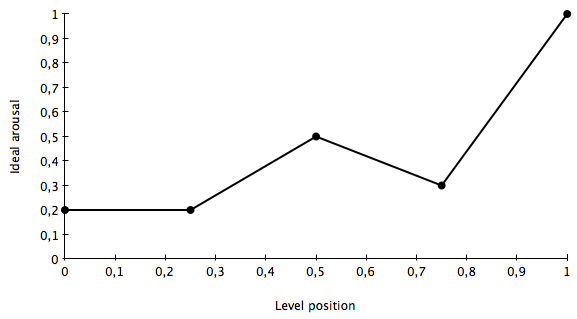
\includegraphics[scale=0.4]{idealGraph.png}
\caption{The intended arousal over the course of the level}
\label{fig:ideal}
\end{figure}
Thus the challenge was to provide a mapping between level features and player arousal. To enable this, we produced an experimental setup where each player would play two levels.
The first would serve as a learning session for establishing the player's arousal responses to different level features. The second would use this information to generate the adapted level.

\subsection{Screen-Chunks and Chunks}
In order to procedurally generate levels for Mario we needed a method for configuring individual tiles into levels.% in a way that would motivate gameplay with varying degrees of complexity, with the underlying assumption that this would lead to varying degress of difficulty and hence engagement and arousal.
Though levels are fundamentally configured of tiles, the individual tile is not necessarily the best level for describing the challenges that the player faces in the game. A tile is quickly traversed by Mario, and the difficulty of doing so can only be determined by looking at neighbouring tiles.

We decided to understand particular configuration of tiles, or chunks of tiles, as the fundamental unit of challenges that the player faces in the game.
The guiding principle for defining a chunk was to look at configurations of tiles that necessitate the player to perform one action, or one combination of actions, to traverse the configuration: for instance jumping over a gap, or upon an enemy to kill it.

Additionally, we defined the concept of screen-chunks: configurations of chunks that are close enough so the actions connected to the chunks influence each other: e.g a jump over one chunk making Mario land on a second chunk, near an enemy that he must kill or avoid.

Levels were constructed by connecting screen-chunks until a desired level width was achieved. For each screen-chunk, windows for Mario's entry and exit were defined. The windows were required to overlap in neighbouring screen-chunks.

The chunks and screen-chunks were designed manually with a custom editor and compiled into a screen-chunk library.
It fell to the human designer to ensure that chunks and screen-chunks were passable by the rules of the game.
During the design process we tried to ensure a variety of complexity and difficulty in the library. These evaluations were solely based on the expertise of the designer.

Each screen-chunk had a related weight that represented its assumed potential for generating arousal. For random levels this was ignored while for adapted levels the weights were used to select the order of screen-chunks.

\subsubsection{Generating Screen-Chunk Weights}
During playthrough of randomly generated levels, arousal responses as expressed by skin conductivity levels from the player were continuosly sampled at a rate of 30Hz, and mapped to the corresponding screen-chunks.

Before any attempts at adaptivity were done, two reference players were asked to play through a multitude of randomly generated levels, collecting a dataset of 490 observations of arousal responses to screen-chunks distributed across the library.%[INDSÆT INFO HER, HVIS VI GIDER]
The observations were then used to train an artificial neural network regressor to predict arousal values for the individual screen-chunks in the library.

Further observations were constructed from the first playthrough of the learning level. They were then used to further train the ANN from its baseline state toward a personalized state.

Finally, this new adapted ANN was used to predict personal weights for every screen-chunk in the library. This updated library then formed the basis for generating personal, adapted levels.

\subsubsection{SCL sampling and treatment}
Preliminary work for the experiments was done using a wireless physiological measurement device called the Empatica E2 \cite{empatica}.
However, we experienced device failure over the course of the project and subsequently psychophysiological sampling was conducted with a Wild Divine Lightstone Biofeedback device which connects via USB \cite{wilddivine}.

The Lighstone device is capable of sampling SCL and BVP at a rate of 32Hz. In this case we only used the SCL signal.
Samples were taken from the three leftmost fingertips of the player's left hand using dry electrodes. The controls of the game were adapted to minimize the inconvenience of wearing the Lightstone while playing.

%Using the publicly available jlsm software package [reference here], w
We interfaced the game engine with sampling software allowing us to fuse sample data with gameplay data from the Mario Framework in real-time.

Before play start, the player went through a 30s period of baseline measurement viewing a blue screen with a countdown.
Once the level started, each sample was tagged with the horizontal position of Mario in the level at sample time. 

Though we were not able to precisely measure the latency from device sampling to in-game location mapping we assumed this to be low enough to be negligible.
The width of the screen-chunks allowed us to assume that most skin conductivity responses to in-game events, in a given screen, would be mapped to the relevant screen-chunk.

After each playthrough, the raw samples of SCL levels were subjected to smoothing by a simple moving average to remove noise from the signal.
The full signal, including the baseline, was then scaled to values between 0 and 1. Subsequently the mean SCL value for each screen-chunk in the level was calculated, as well as the maximum value measured during time spent in that screen chunk.

Finally, for each screen-chunk that the player had experienced in the level, an observation was generated.
Each observation consisted of the count of individual chunks in the screen-chunk, and the mean SCL value.
These observations were then used as training examples for the ANN regressor that in turn was used to predict screen-chunk arousal induction potential.

\subsection{Results}
A number of network topologies were attempted multiple times. The best performing one was a 3-2 hidden layer topology, trained for 100.000 epochs. The ANN regressor exhibited a correlation coefficient of 0,3122 between expected and produced values and a relative absolute error of ca. 89\%. Though this performance was slightly discouraging, we proceeded to use the network for a pilot run of four user tests.

Two of these players did not manage to complete the personalized levels, arguably because the generated level was unfit for their skill level.
The two other players completed their personalized levels. Their arousal responses to the random and personalized levels are included in in figures \ref{fig:playerFirst} and \ref{fig:playerLast}.

Since it was impossible to, within the scope of this project, collect a data material suitable for extensive statistical analysis, we instead opted to present these preliminary results on a case-by-case basis and consider this project a pre-pilot for the actual testing of the solution.

For the method to be considered successful, we would require the curves of the personalized sessions to conform, at least to some extent, to the chosen ideal curve presented earlier in figure \ref{fig:ideal}.

While none of the signals correspond clearly to the curve we tried to induce, we find it worth noticing that both players exhibit spikes of arousal activity at the middle of the level, followed by drops in arousal, which are then followed by a second spike in activity at the end of the personalized level.
However, we also see patterns of spikes completely seemingly unrelated to the desired arousal curve.

\begin{figure}
\centering
\includegraphics[scale=0.4]{movieStar.png}
\caption{Player I}
\label{fig:playerFirst}
\end{figure}
\begin{figure}
\centering
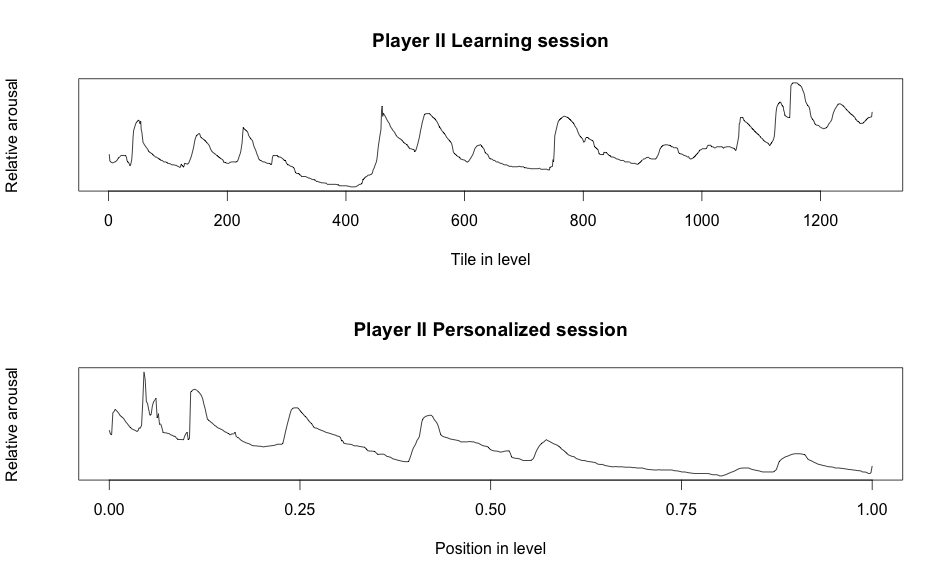
\includegraphics[scale=0.4]{nicklas.png}
\caption{Player II}
\label{fig:playerLast}
\end{figure}

\section{Discussion}
Our solution for procedurally generating levels based on expected values suffered from a number of issues that would need to be further improved and/or investigated in order to test for evidence for the success of the generator:
\begin{description}
\item [The signal treatment] employed in the solution was relatively na\"{\i}ve, and the literature suggests a multitude of methods that would be worth applying to see if a more robust performance could be achieved.
Drift correction, signal deconvolution, extraction of the phasic driver from the general SCL signal, artefact correction, and more advanced peak detection are all analytical procedures that could be added to the signal treatment. The original Empatica device that failed features deconvolution and SCL driver extraction in firmware while the Lightstone device does not. Once the fail occurred, time did not permit for implementing these features in software.

Additionally, employing a multimodal approach, fusing other ordered time series of signals with the SCL signal could perhaps improve the efficiency of the approach\cite{martinez2011mining}. This could include other physiological measurements, such as BVP, but could also include series of data representing player inputs or game events.
A third option for generating an auxiliary signal could be to analyse the difficulty of the screen-chunks using an AI agent.
Prior research indicates that this approach, combined with sequence mining, can yield useful results \cite{martinez2011mining}.% Unfortunately, the implementation of such more advanced techniques fell outside of the scope of this project.
\item [Classifier/regressor accuracy] could have been improved in several different manners. Obviously, a larger data set for the training the ANN would have been preferable. Other machine learning methods could have been applied, e.g. NEAT or regression/decision trees \cite{liu2009dynamic}.
\item [Training data sets] could have been larger, given the opportunity to collect more data from additional respondents.
The simplistic approach of training the baseline ANN on data from only two persons is a questionable approach and should optimally be replaced with hours upon hours of gameplay from many different individuals.
\item [The screen-chunk library] could have been extended to include more screen-chunks, in turn allowing for more variety in the configurations of individual chunks - or a more automated approach to screen-chunk generation could have been applied \cite{shaker2011feature}.
This would in turn have provided us with the opportunity of generating a better training set for the ANN. However, in lieu of the low number of training observations that we could feasibly generate within the available time frame, this was not a practical issue.
\end{description}
At the general level, however, we must also question the appropriateness of the use of arousal data for off-line adaptive content generation.
\begin{description}
\item [The arousal-engagement assumption] is well-grounded in the literature, but for this particular experiment, we did not include any source of external ground truth, or a second corroborating measure of player engagement. This would have been beneficial and should be included in future studies.
\item [Player skill and play style] are not taken directly into account in the current model, only to the extent that frustration from failing or overcoming great challenges would be expected to increase arousal. Working with a less tacit understanding of player skill and style, and using this as separate vectors of information about the player's interaction, as described in the literature \cite{shaker2010towards}, could probably be a valuable improvement to the overall approach.
\item [Habituation/player learning] over the course of play is not addressed in the current model of generation. Specifically, one participant (Player II) told us, that he subjectively experienced a strong learning effect. While the screen-chunks at the end of the personalized level were indeed challenging to him when he first met them, he quickly learned to defeat the screen-chunk and hence stopped considering it challenging. This meant that his learning likely invalidated the weights in the screen-chunk library (assuming they were ever valid) \emph{over the course of a single playthrough}.
This in turn raises the point that it is possible that any practical implementation of this general approach for PCG should be continuously monitoring, analysing, and updating its player model online, during play, rather than between sessions.
\end{description}

\section{Conclusion and future work}
The project presented here has been a first investigation into the use of physiological signals to drive adaptive content in platform games.
The specific implementation was, due to constraints of time and scope, unable to produce sufficient evidence to draw any conclusions about the usefulness of the approach.
It should probably best be considered a feasibility study or a pre-pilot to a study, since it is limited by aspects of data treatment and sample sizes.

We do however consider the project to have shown that a more extensive study using the same principles, with the improvements outlined in the discussion above, \emph{might} provide valuable knowledge on the usefulness of psychophysiology for the generation of content for platform games.

In the case that robust measurement devices become integrated components in consumer-grade gaming equipment, it would not be far fetched that this vein of affective computing could find a use in commercial games, and this project demonstrates that it would be within the reach of even minor productions to test the usefulness of the approach for specific games during development.

\bibliography{references}
\end{document}